\documentclass[reprint,amsmath,amssymb,aps]{revtex4-2}

\usepackage[utf8]{inputenc}
\usepackage[T1]{fontenc}
\usepackage{physics}
\usepackage{graphicx}
\usepackage{dcolumn}
\usepackage{multirow}
\usepackage{booktabs}
\usepackage{float}
\usepackage{bm}
\usepackage{makecell}
\usepackage{siunitx}
\usepackage{hyperref}

\begin{document}
	
	\title{Interpolación de Lagrange e integración numérica clásica aplicadas al análisis de trayectorias orbitales}
	
	\author{Juan Carlos Celis Lozada}
	\email[]{juan.celisloz@unipamplona.edu.co}
	\affiliation{Universidad de Pamplona, Programa de Física, Pamplona, Norte de Santander, Colombia}
	
	\date{\today}
	
	\begin{abstract}
		La interpolación polinómica es una herramienta fundamental en el análisis numérico para la reconstrucción de funciones a partir de datos discretos, con aplicaciones directas en problemas físicos y astrodinámicos. En este trabajo se analiza el desempeño de la interpolación polinómica de Lagrange aplicada a trayectorias orbitales elípticas descritas por una expresión Kepleriana. Se implementa un procedimiento computacional en Python para muestrear la órbita, reconstruirla mediante un polinomio interpolante global y cuantificar el error geométrico en función del número de nodos y de la excentricidad orbital. Asimismo, se evalúa el impacto de la interpolación en cálculos posteriores de integración numérica, comparando los valores de la integral radial obtenidos a partir de la órbita analítica y de la órbita interpolada mediante la regla de Simpson y la cuadratura de Gauss--Legendre. Los resultados muestran que la precisión de la interpolación depende críticamente de la discretización y de la geometría orbital, evidenciándose oscilaciones asociadas al fenómeno de Runge para mallas equiespaciadas. A pesar de ello, las integrales numéricas calculadas a partir de la función interpolada presentan discrepancias relativas inferiores al $0.1\%$, lo que pone de manifiesto la robustez de los métodos de cuadratura frente a errores moderados en la función de entrada.
	\end{abstract}
	
	\keywords{Interpolación de Lagrange; Aproximación polinómica; Trayectorias orbitales; Error numérico; Integración de Simpson; Cuadratura de Gauss--Legendre}
	
	\maketitle
	
	\section{Introducción}
	
La interpolación de funciones es un procedimiento fundamental en el análisis numérico, utilizado para aproximar una función desconocida a partir de un conjunto finito de datos experimentales o calculados. Entre los métodos más empleados se encuentra la interpolación polinómica, cuya formulación clásica puede encontrarse en los textos estándar de cálculo numérico \cite{BurdenFaires, Atkinson}.

El método de interpolación de Lagrange permite construir un único polinomio de grado máximo $n$, capaz de pasar exactamente por $n+1$ puntos dados. Este enfoque, introducido de manera formal en los estudios de aproximación e interpolación \cite{Runge1901}, constituye uno de los pilares teóricos para el análisis de errores y estabilidad en la aproximación polinómica. Su utilidad radica en su formulación explícita, que facilita el análisis matemático y la comprensión del comportamiento de los polinomios en mallas arbitrarias.

No obstante, la interpolación polinómica global presenta limitaciones importantes, entre ellas el crecimiento del error en mallas equidistantes, fenómeno identificado y analizado en profundidad en estudios clásicos de la teoría de aproximación \cite{Trefethen2013}. Esta problemática ha dado lugar a desarrollos teóricos y prácticos orientados a seleccionar conjuntos óptimos de nodos o a emplear interpolación por partes.

Desde el punto de vista computacional, la implementación directa de la fórmula de Lagrange no siempre es la estrategia más eficiente. Análisis numéricos detallados sobre estabilidad y precisión muestran que el cálculo explícito de los polinomios base puede resultar costoso y propenso a errores de redondeo \cite{NumericalRecipes}. No obstante, para fines analíticos, de visualización o de desarrollo teórico, su estructura cerrada sigue siendo de gran relevancia.

En este trabajo se desarrolla la formulación explícita del método de interpolación de Lagrange y se presenta un estudio ilustrativo basado en datos discretos, con el propósito de analizar su comportamiento y comprender las implicaciones prácticas de este procedimiento clásico.
	
	\section{Detalles computacionales}
	
	El estudio numérico desarrollado en este trabajo se apoya en un conjunto de rutinas implementadas en el lenguaje Python, cuyo objetivo es analizar el comportamiento de la interpolación polinómica de Lagrange aplicada a trayectorias orbitales y evaluar su impacto en cálculos posteriores de integración numérica. El enfoque computacional se estructura de manera secuencial, partiendo de la definición de una órbita analítica de referencia y avanzando hacia la reconstrucción interpolada, la cuantificación del error geométrico y la comparación entre distintos esquemas de cuadratura.
	
	La órbita de referencia se genera a partir de la expresión Kepleriana para una trayectoria elíptica en coordenadas polares,
	\begin{equation}
		r(\theta)=\frac{a(1-e^{2})}{1-e\cos\theta},
		\label{eq:kepler}
	\end{equation}
	donde $a$ representa el semieje mayor y $e$ la excentricidad orbital. A partir de la ecuación~\eqref{eq:kepler} se obtienen las componentes cartesianas de la órbita mediante las transformaciones
	\begin{align}
		x(\theta) &= r(\theta)\cos\theta, \label{eq:xcoord}\\
		y(\theta) &= r(\theta)\sin\theta. \label{eq:ycoord}
	\end{align}
	Estas expresiones permiten construir una representación completa de la trayectoria en el plano. Para garantizar una referencia numérica precisa, se emplea una malla angular densa en el intervalo $[0,2\pi]$, la cual se considera como la solución analítica frente a la cual se evalúan los errores de interpolación.
	
	El muestreo discreto de la órbita se realiza seleccionando un número finito $N$ de nodos equiespaciados en la variable angular $\theta$. A partir de las ecuaciones~\eqref{eq:xcoord} y~\eqref{eq:ycoord} se extraen los valores discretos $(\theta_i,x_i,y_i)$, los cuales constituyen la información disponible para la reconstrucción interpolada. El parámetro $N$ se controla explícitamente en el código, permitiendo estudiar de manera sistemática su influencia sobre la precisión geométrica del ajuste.
	
	La interpolación se lleva a cabo mediante el polinomio de Lagrange global. Para una función genérica $f(\theta)$, el polinomio interpolante se define como
	\begin{equation}
		P(\theta)=\sum_{i=0}^{N-1} f(\theta_i)\,\ell_i(\theta),
		\label{eq:lagrange_poly}
	\end{equation}
	donde las funciones base de Lagrange están dadas por
	\begin{equation}
		\ell_i(\theta)=\prod_{\substack{j=0 \\ j\neq i}}^{N-1}
		\frac{\theta-\theta_j}{\theta_i-\theta_j}.
		\label{eq:lagrange_basis}
	\end{equation}
	Las ecuaciones~\eqref{eq:lagrange_poly} y~\eqref{eq:lagrange_basis} se aplican de forma independiente a las componentes $x(\theta)$ y $y(\theta)$, permitiendo reconstruir la trayectoria completa a partir de los nodos discretos. El polinomio interpolante se evalúa posteriormente sobre una malla angular fina para compararlo con la órbita analítica original.
	
	La cuantificación del error geométrico se realiza mediante la distancia euclidiana entre la curva interpolada y la curva analítica, definida como
	\begin{equation}
		\varepsilon(\theta)=\sqrt{
			\left(x_{\text{interp}}-x_{\text{real}}\right)^2+
			\left(y_{\text{interp}}-y_{\text{real}}\right)^2}.
		\label{eq:error}
	\end{equation}
	La ecuación~\eqref{eq:error} permite obtener tanto el perfil del error a lo largo de la órbita como valores característicos, entre ellos el error máximo y el error cuadrático medio. Este análisis resulta particularmente relevante en regiones cercanas al periastro, donde la variación de la función radial es más abrupta.
	
	Para estudiar de forma diferenciada los factores que influyen en la interpolación, se realizan varios experimentos numéricos. En el primero se varía el número de nodos $N$ manteniendo fija la excentricidad orbital, lo que permite evaluar el efecto de la discretización sobre la calidad del ajuste. En el segundo, se fija el número de nodos y se modifica la excentricidad, con el objetivo de analizar cómo la geometría de la órbita condiciona el desempeño del polinomio interpolante definido en la ecuación~\eqref{eq:lagrange_poly}. Adicionalmente, se considera un caso particular con excentricidad elevada ($e=0.8$), para el cual se comparan distintas cantidades de nodos en una sola visualización, facilitando la identificación del rango de valores de $N$ para los cuales la interpolación reproduce de manera más fiel la trayectoria analítica.
	
	Finalmente, se evalúa el impacto de la interpolación en cálculos de integración numérica. Se considera la integral radial
	\begin{equation}
		I=\int_{0}^{2\pi} r(\theta)\,d\theta,
		\label{eq:integral}
	\end{equation}
	la cual se calcula tanto utilizando la función analítica definida en la ecuación~\eqref{eq:kepler} como su versión reconstruida mediante interpolación. La integral~\eqref{eq:integral} se evalúa empleando la regla de Simpson compuesta y la cuadratura de Gauss--Legendre de orden finito. La comparación entre los valores obtenidos permite cuantificar el sesgo introducido por la interpolación y evaluar la robustez de ambos métodos de cuadratura frente a errores en la función de entrada.
	
	Las rutinas desarrolladas generan de forma automática las gráficas de las órbitas reales e interpoladas, los perfiles del error geométrico definido en la ecuación~\eqref{eq:error} y las tablas comparativas de los valores integrales, las cuales constituyen la base del análisis presentado en la sección de resultados.
	
	
	
	\section{Resultados}
	
	La interpolación polinómica de Lagrange definida en la ecuación~\eqref{eq:lagrange_poly} se aplicó a la órbita kepleriana dada por la ecuación~\eqref{eq:kepler}. La Fig.~\ref{fig:orbita5} muestra la reconstrucción orbital obtenida con un número reducido de nodos ($N=5$), donde se observan desviaciones significativas respecto a la trayectoria analítica. Al incrementar el número de nodos, la aproximación mejora sustancialmente, como se evidencia en la Fig.~\ref{fig:orbita25}. No obstante, el perfil del error euclidiano revela oscilaciones asociadas al fenómeno de Runge (Fig.~\ref{fig:error25}).
	
	\begin{figure}[H]
		\centering
		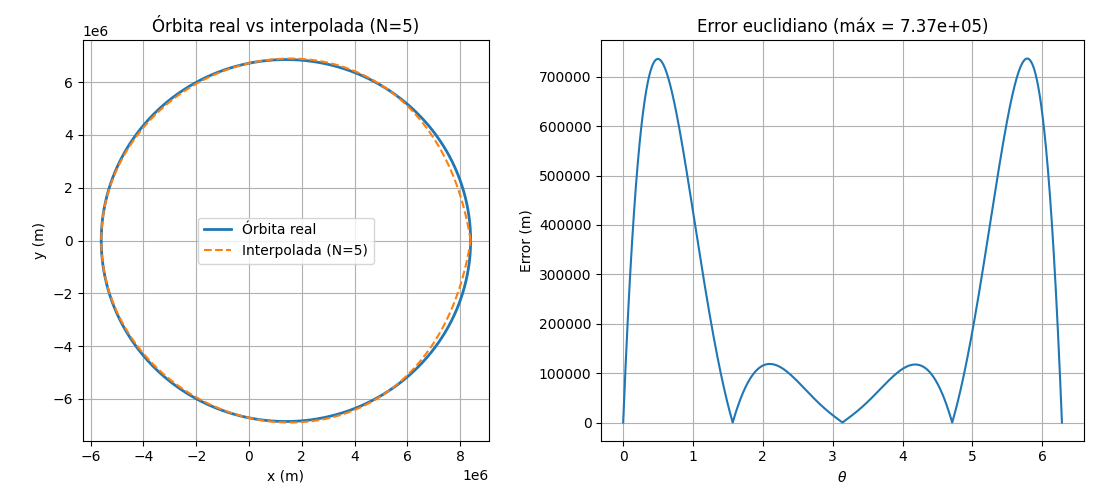
\includegraphics[width=0.45\textwidth]{resultado1.png}
		\caption{Órbita analítica e interpolada (izquierda) y error euclidiano (derecha) para $N=5$ nodos.}
		\label{fig:orbita5}
	\end{figure}
	
	\begin{figure}[H]
		\centering
		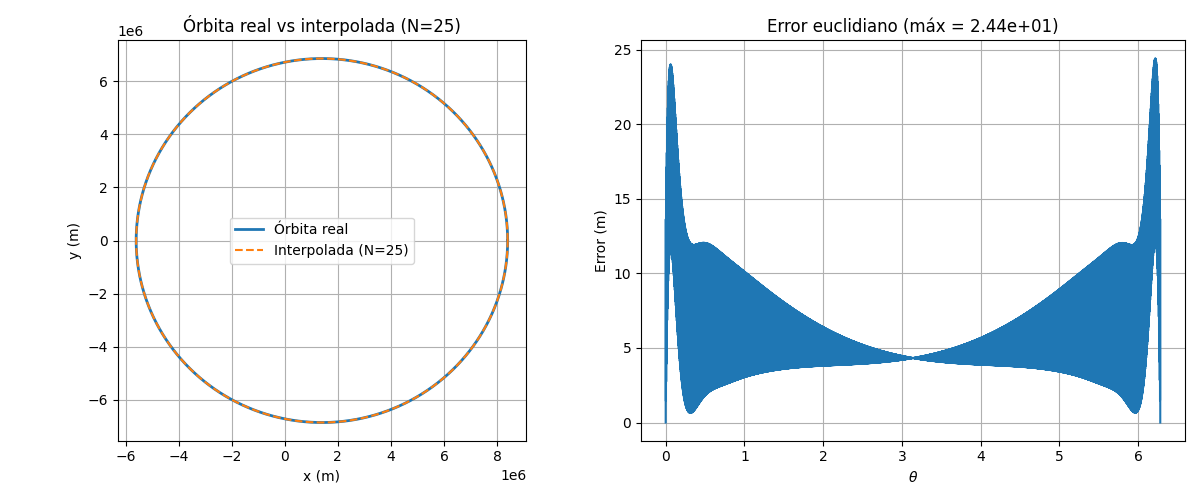
\includegraphics[width=0.45\textwidth]{resultado11.png}
		\caption{Órbita analítica e interpolada (izquierda) y error euclidiano (derecha) para $N=25$ nodos.}
		\label{fig:orbita25}
	\end{figure}
	
	\begin{figure}[H]
		\centering
		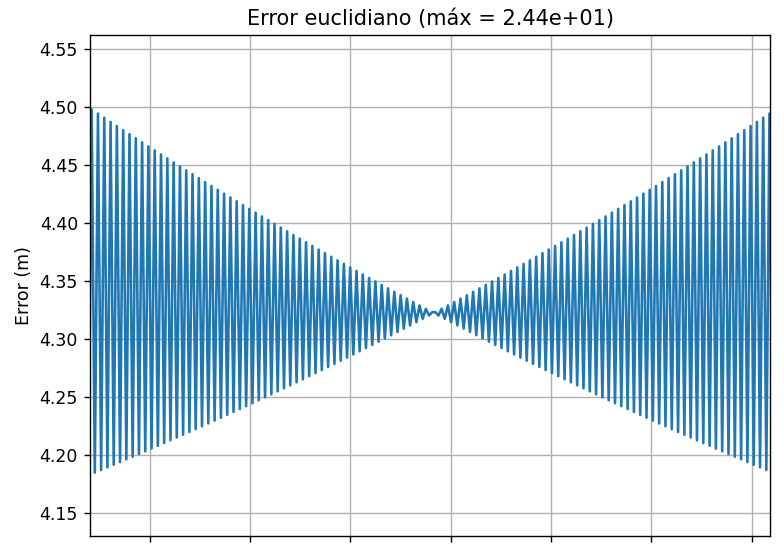
\includegraphics[width=0.45\textwidth]{runge.png}
		\caption{Oscilaciones del error euclidiano asociadas al fenómeno de Runge para $N=25$ nodos.}
		\label{fig:error25}
	\end{figure}
	
	El efecto de la excentricidad orbital sobre la interpolación se presenta en la Fig.~\ref{fig:excentricidades}, donde se observa un incremento progresivo del error al aumentar $e$ para un número fijo de nodos ($N=15$). Para órbitas altamente excéntricas ($e=0.8$), la precisión del ajuste depende fuertemente de la cantidad de nodos, como se muestra en la Fig.~\ref{fig:elipticasnodos}.
	
	\begin{figure}[H]
		\centering
		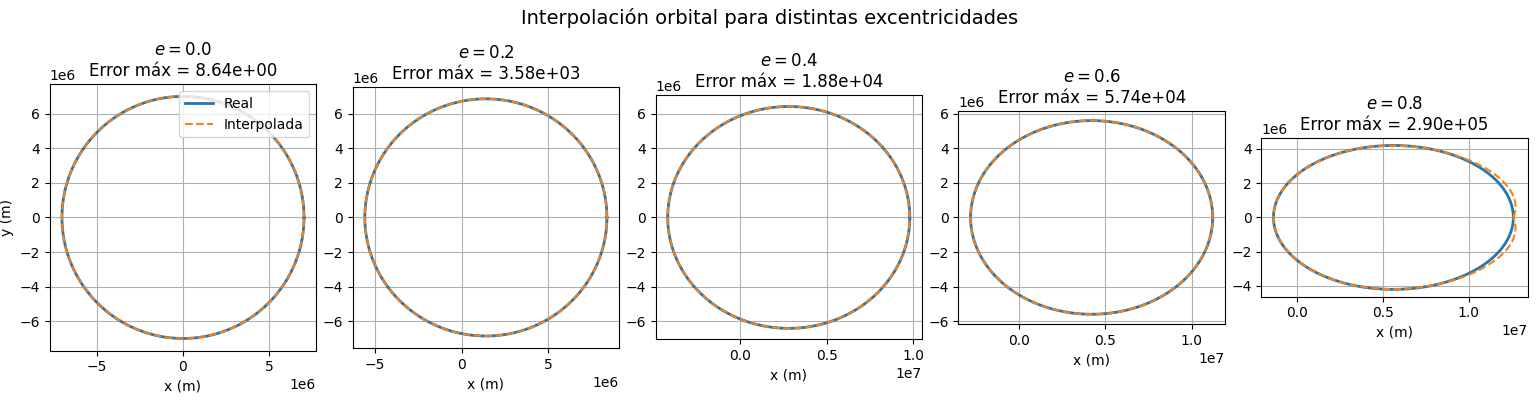
\includegraphics[width=0.45\textwidth]{Excentricidad.png}
		\caption{Órbita real e interpolada para distintas excentricidades con $N=15$ nodos.}
		\label{fig:excentricidades}
	\end{figure}
	
	\begin{figure}[H]
		\centering
		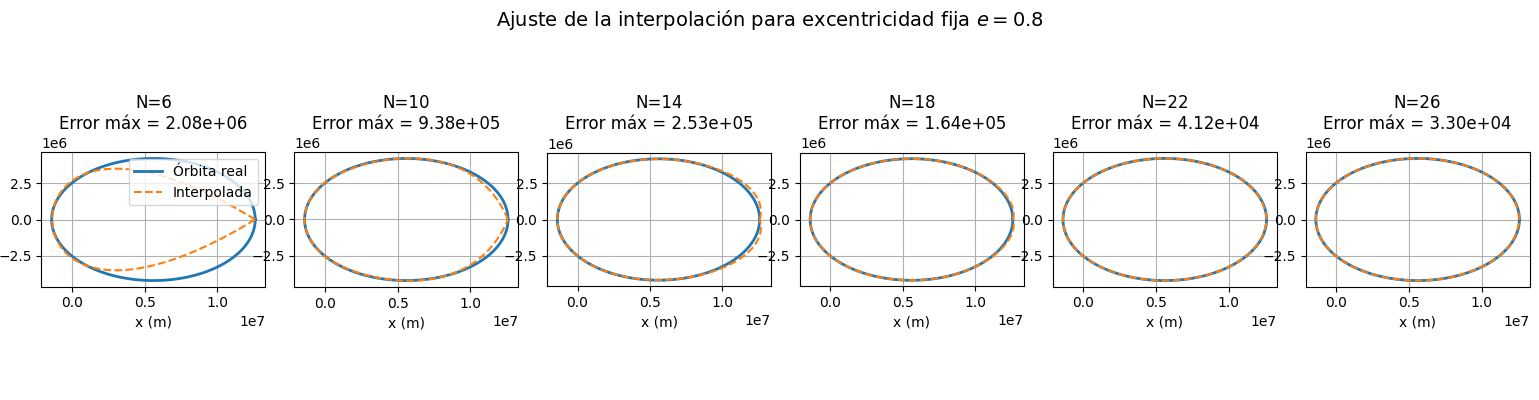
\includegraphics[width=0.45\textwidth]{excentricidad nodos.png}
		\caption{Órbita real e interpolada para $e=0.8$ y distintos números de nodos.}
		\label{fig:elipticasnodos}
	\end{figure}
	
	La Tabla~\ref{tab:integracion} presenta la comparación entre la integral radial definida en la ecuación~\eqref{eq:integral}, evaluada a partir de la órbita analítica y de la órbita interpolada. Para ambos métodos de integración, las diferencias absolutas se mantienen del orden de $10^{4}$, con errores relativos inferiores al $0.1\%$.
	
	\begin{table}[H]
		\centering
		\begin{tabular}{ccccc}
			\toprule
			Método & \makecell{Integral\\analítica} & \makecell{Integral\\interpolada} & Diferencia & \% Error \\
			\midrule
			Simpson & $2.6389\times 10^{7}$ & $2.6403\times 10^{7}$ & $1.3857\times 10^{4}$ & 0.054 \\
			\makecell{Gauss--\\Legendre} & $2.6359\times 10^{7}$ & $2.6383\times 10^{7}$ & $2.4636\times 10^{4}$ & 0.091 \\
			\bottomrule
		\end{tabular}
		\caption{Comparación entre la integral radial real y la interpolada utilizando Simpson y Gauss--Legendre.}
		\label{tab:integracion}
	\end{table}
	
	
	
	\section{Conclusiones}
	
	Se analizó la interpolación polinómica de Lagrange aplicada a trayectorias orbitales elípticas y su efecto en cálculos geométricos e integrales. Los resultados muestran que la precisión de la reconstrucción depende críticamente del número de nodos y de la excentricidad orbital. Para mallas poco densas, el error geométrico es significativo y se manifiestan oscilaciones asociadas al fenómeno de Runge, mientras que un incremento adecuado de nodos permite una aproximación estable de la trayectoria.
	
	Asimismo, se observó que el aumento de la excentricidad deteriora la calidad de la interpolación global, particularmente en regiones cercanas al periastro, donde la variación de la función radial es más pronunciada. En órbitas altamente excéntricas, la elección del número de nodos resulta determinante para reproducir correctamente la geometría orbital.
	
	En cuanto a la integración numérica, las integrales evaluadas a partir de la órbita interpolada presentan un sesgo sistemático pequeño respecto a la solución analítica. Las diferencias obtenidas mediante la regla de Simpson y la cuadratura de Gauss--Legendre se mantienen por debajo del $0.1\%$, lo que evidencia la robustez de estos métodos frente a errores moderados en la función integrada. En conjunto, los resultados confirman que la interpolación de Lagrange puede emplearse con éxito en aplicaciones astrodinámicas siempre que se controle adecuadamente la discretización y la complejidad geométrica de la órbita.
	
	
	
	
	
	\begin{thebibliography}{99}
		
		\bibitem{BurdenFaires}
		R. L. Burden and J. D. Faires,
		\textit{Numerical Analysis},
		Cengage Learning (2011).
		
		\bibitem{Atkinson}
		K. Atkinson,
		\textit{An Introduction to Numerical Analysis},
		Wiley (1989).
		
		\bibitem{Runge1901}
		C. Runge,
		``Über empirische Funktionen und die Interpolation zwischen äquidistanten Ordinaten,''
		Zeitschrift für Mathematik und Physik \textbf{46}, 224–243 (1901).
		
		\bibitem{Trefethen2013}
		L. N. Trefethen,
		\textit{Approximation Theory and Approximation Practice},
		SIAM (2013).
		
		\bibitem{NumericalRecipes}
		W. Press, S. Teukolsky, W. Vetterling, and B. Flannery,
		\textit{Numerical Recipes}, 
		Cambridge University Press (2007).
		
	\end{thebibliography}
	
	\section{Anexos}
	\begin{figure}[H]
		\centering
		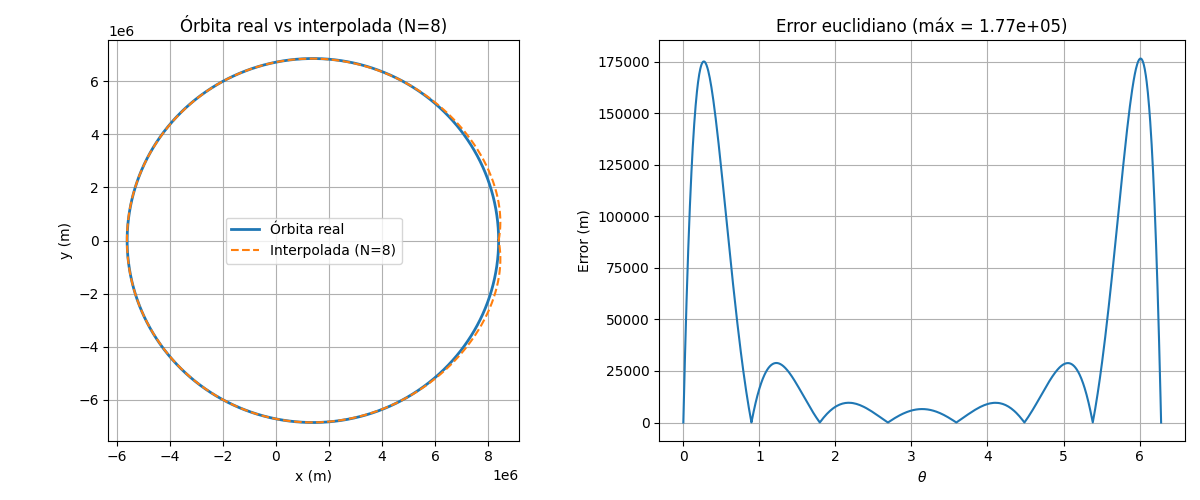
\includegraphics[width=0.5\textwidth]{resultado3.png}
		\caption{Órbita real e interpolada (izquierda) y su error euclidiano (derecha) con $N=8$ nodos.}
		\label{fig:orbita8}
	\end{figure}
	
	
	\begin{figure}[H]
		\centering
		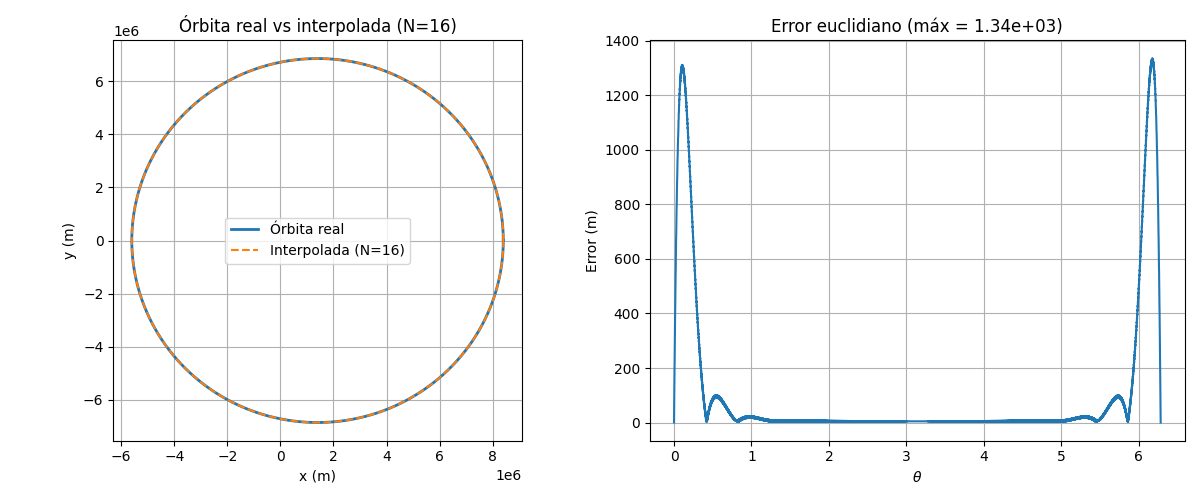
\includegraphics[width=0.5\textwidth]{resultado7.png}
		\caption{Órbita real e interpolada (izquierda) y su error euclidiano (derecha) con $N=16$ nodos.}
		\label{fig:orbita16}
	\end{figure}
	
\end{document}

